\documentclass[tikz, margin=3.14mm]{standalone} 
\usetikzlibrary{calc,angles,quotes,arrows.meta}

\tikzset{pill/.style={minimum width=1.2cm,minimum height=6mm,rounded
corners=3mm,draw},
reactor/.style={circle,draw,minimum size=6mm,path picture={
\draw (-3mm,0) -- (3mm,0) (0,-3mm) -- (0,3mm);
\fill (0,0) -- (3mm,0) arc(0:-90:3mm) -- cycle;
\fill (0,0) -- (-3mm,0) arc(180:90:3mm) -- cycle;
}}}

\begin{document}    
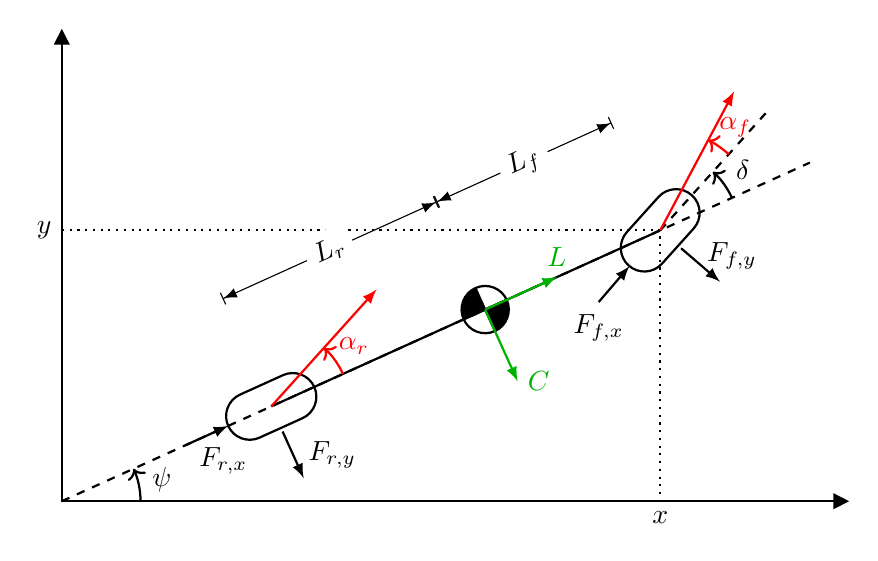
\begin{tikzpicture}
\draw[thick,{Triangle[length=2mm]}-{Triangle[length=2mm]}] (0,6) coordinate (Y) -- (0,0) coordinate (O)-- (10,0)
coordinate (X);
\draw[thick,dashed] (O) -- (9.5,4.3) coordinate[pos=0.28] (F1) coordinate[pos=0.8] (F2) coordinate (TR);
\draw[thick,dotted] (O |- F2) node[left]{$y$} -- (F2) -- (O -| F2) node[below] {$x$};
\draw[thick] (F1)  -- (F2) node[pos=0.55,sloped,reactor] (M){~}
node[pos=0,sloped,pill]{};
\draw[green!70!black,thick,-latex] (M.center) -- ($(M.center)!1cm!0:(F2)$)
node[above]{$L$};
\draw[green!70!black,thick,-latex] (M.center) -- ($(M.center)!-1cm!90:(F2)$)
node[right]{$C$};
\draw[thick,dashed] (F2) -- ++ (48:2) coordinate(H)  node[pos=0,sloped,pill,solid]{}
pic ["$\delta$",draw,solid,->,angle radius=1cm,angle eccentricity=1.3] {angle = TR--F2--H};
\draw[thick,red,-latex] (F2) -- ++ (62:2) coordinate (A2) node[below=0.46cm,right=-0.32cm]{$\alpha_f$}
pic [draw,->,red,thick,angle radius=1.3cm] {angle = H--F2--A2};
\draw[thick,red,-latex] (F1) -- ++ (48:2) coordinate (A1)
pic ["$\alpha_r$",draw,->,red,thick,angle radius=1cm,angle eccentricity=1.3] {angle = F2--F1--A1};
% rear forces
\draw[latex-,thick] ($(F1)!10mm!-90:(M)$) -- ($(F1)!3.5mm!-90:(M)$) node[below=0.3cm,right=0.2cm]{$F_{r,y}$};
\draw[latex-,thick] ($(F1)!-6mm!0:(M)$) -- ($(F1)!-12mm!0:(M)$) node[below=0.2cm,right=0.05cm]{$F_{r,x}$};

% front forces
\draw[latex-,thick] ($(F2)!10mm!115:(M)$) -- ($(F2)!3.5mm!115:(M)$) node[below=0.1cm,right=0.2cm]{$F_{f,y}$};
\draw[latex-,thick] ($(F2)!6mm!25:(M)$) -- ($(F2)!12mm!25:(M)$) node[below=0.03cm]{$F_{f,x}$};

\draw[{Bar}{Latex}-{Latex}{Bar}] ($(F1)!1.5cm!90:(M)$) -- 
($(M)!1.5cm!90:(F2)$) node[midway,sloped,fill=white]{$L_r$};
\draw[{Bar}{Latex}-{Latex}{Bar}] ($(M)!1.5cm!90:(F2)$) -- 
($(F2)!1.5cm!-90:(M)$) node[midway,sloped,fill=white]{$L_f$};

\draw[thick,black,-latex]
pic ["$\psi$",draw,->,black,thick,angle radius=1cm,angle eccentricity=1.3] {angle = X--O--F1};
\end{tikzpicture}
\end{document}